% Crucible v1 — arXiv manuscript
% Compile: cd paper && tectonic main.tex
% Every number in this file is copied from paper/REANALYSIS.md (regenerated by
% crucible/tools/reanalysis.js) or paper/INVENTORY.md (crucible/tools/inventory.js); both are
% checked in CI against the frozen ledgers in crucible/results/. Figures are TikZ emitted by the
% same scripts. Do not hand-edit numbers here without re-running the generators.
\documentclass[10pt]{article}
\usepackage[margin=1in]{geometry}
\usepackage[T1]{fontenc}
\usepackage{newtxtext,newtxmath}
\usepackage{microtype}
\usepackage{booktabs}
\usepackage{multirow}
\usepackage{graphicx}
\usepackage{xcolor}
\usepackage{amsmath}
\usepackage{pgfplots}
\pgfplotsset{compat=1.18}
\definecolor{figblue}{HTML}{0072B2}
\definecolor{figvermilion}{HTML}{D55E00}
\definecolor{figgreen}{HTML}{009E73}
\definecolor{figpink}{HTML}{CC79A7}
\usepackage[numbers,sort&compress]{natbib}
\usepackage[colorlinks=true,linkcolor=blue!60!black,citecolor=blue!60!black,urlcolor=blue!60!black]{hyperref}
\usepackage{enumitem}
\setlist{itemsep=1pt,topsep=2pt,parsep=0pt}
\usepackage{appendix}

\newcommand{\goodput}{\textsc{Goodput}}
\newcommand{\crucible}{\textsc{Crucible}}
\newcommand{\pair}[2]{\texttt{#1}\,@\,\texttt{#2}}
\newcommand{\ci}[2]{[#1,\,#2]}

\title{\textbf{\crucible{}: An Empirical Study of Harness--Model Compatibility\\ and Delivery in Local Coding Agents}}

\author{%
  Siddhant Goswami\\
  100x Engineers, Bengaluru, India\\
  \texttt{content@100xengineers.com}%
}
\date{}

\begin{document}
\maketitle

\begin{abstract}
A coding agent is a configuration: a model plus the harness that turns it into an agent (prompt
assembly, tools, the execution loop, verification, recovery, permissions). We ask, under fixed
task and resource conditions, how the configuration affects \emph{delivery}---a verifier pass
within a stated deadline---and what observable failures explain the rest. \crucible{} is a
small apparatus for that question: a one-line adapter contract, a bounded act$\to$verify loop
owned by the runner, deterministic hidden verifiers, uniform token metering, and frozen run
ledgers from which every reported number regenerates in CI. We report 1{,}448 attempted runs
across five local cohorts (seven harnesses; six local models in three families) plus small
cloud slices. Three findings survive a reanalysis on matched task sets with task-clustered
intervals. (i)~Within a model column, harness choice moves delivery from 0.00 to 0.89 on
\texttt{qwen3:8b}, but only two of the pre-named within-model contrasts are significant under
both delivery and the gated score; three others are significant under one metric only, and we
show which. (ii)~Holding weights fixed on \texttt{qwen3.5:9b}, one tool-calling harness delivers
0.89 while another delivers 0.00 ($\Delta{=}{+}0.89$ \ci{0.78}{1.00}): the same harness is 0 for
262 of 262 attempted local cells across five cohorts, a protocol failure visible in every trace,
while it delivers 20/20 on its vendor's cloud account. (iii)~Scoring finished runs only reorders
five of six harnesses on \texttt{qwen3:8b}; counting timeouts as failed deliveries is
necessary, but a per-cell autopsy attributes 51 of the pilot's 55 timeouts to host-conditional
wall-clock cutoffs rather than harness hangs. A pre-registered third-family arm reproduces the
structural zero and one directional contrast out of sample; a ten-task Terminal-Bench slice
reproduces the ordering but not significance. The study is exploratory except where marked; its
main limitations are nine authored tasks, one host, and adapted external tasks.
\end{abstract}

\section{Introduction}
\label{sec:intro}

Practitioners who run coding agents on local or mid-tier models choose a harness as much as a
model, and the harness is rarely disclosed when agents are compared
\citep{stopcomparing,scaffoldeffect}. The recent literature agrees that the harness matters:
scaffold swaps move SWE-bench by 10--20 points \citep{swebench,epoch2024benchmarking}, the
agent--computer interface alone unlocked large gains \citep{sweagent}, two scaffolds on one model
disagree on a large fraction of tasks \citep{hal}, a single harness treatment transfers across
frozen models \citep{samemodel}, and Harness-Bench measures model$\times$harness configurations
under shared budgets with a security gate \citep{harnessbench}. What that literature mostly
reports is strong cloud models, on which harness choice moves tokens far more than pass rate
(\citet{scaffoldeffect} find 40$\times$ token variation against 0--8 point pass-rate differences).

This paper is a bounded empirical study in the complementary regime: \emph{small local models}
(1.5B--9.7B parameters on one Apple-Silicon host), where the harness moves the pass rate itself.
It asks one question---under the tested task and resource conditions, how does configuration
affect successful delivery, and what observable failures explain unsuccessful attempts?---and
makes three bounded contributions:

\begin{enumerate}
\item \textbf{A reproducible apparatus} (\S\ref{sec:setup}) for comparing specified
  harness--model configurations: an adapter contract, a runner-owned bounded loop, hidden
  deterministic verifiers restored before every check, a token-metering proxy, and frozen
  ledgers with CI guards that fail the build when any published number, table, or figure
  drifts from the records.
\item \textbf{Configuration-dependent delivery on a bounded task battery}
  (\S\ref{sec:results}): within-model contrasts with task-clustered intervals, a within-family
  size ladder, and a pre-registered out-of-sample arm---each reported under two outcome metrics
  so that metric-dependence is visible rather than hidden.
\item \textbf{A diagnostic account of failures} (\S\ref{sec:failures}): a rule-derived failure
  taxonomy over every attempted cell, a weights-fixed protocol-failure demonstration, a timeout
  autopsy, and safety-gate components reported separately from the composite.
\end{enumerate}

We describe the study as \emph{exploratory} throughout, except for the one arm whose predictions
were frozen before execution (\S\ref{sec:phased}). Broad causal claims---that harness effects
dominate model capability in general, or that a cloud model swap isolates interface
compatibility---are not made here; \S\ref{sec:limits} says why, and Appendix~\ref{app:predictions}
records which pre-registered predictions held, which were refuted, and which were never tested.

\section{Related work}
\label{sec:related}

\textbf{Harness as the variable.} Harness-Bench \citep{harnessbench} is the closest system:
model$\times$harness configurations on 106 tasks under shared budgets, a multiplicative security
gate, and process scoring. \crucible{} shares that design (and cites it as the source of its
factorial protocol and gate) but differs in regime and mechanism: sub-frontier local models as
probes, deterministic trace-derived process scores rather than LLM log analysis, timeouts kept in
the delivery denominator, and a cross-model rank-stability test against a seed-noise null.
\citet{harnessaudit} formalize trajectory-level safety auditing and multiplicative scoring; our T4
tier is a small instance with per-channel deterministic checks. \citet{stopcomparing} argue that
harness-induced variance exceeds model-induced variance and call for disclosure; we do not estimate
that decomposition (it needs a design we lack) but supply the disclosure. \citet{scaffoldeffect}
compare three open-source harnesses on two strong models and find large token but small pass-rate
effects; our local-model regime is where the pass-rate effect appears, which is the intended
complement. \citet{samemodel} show one harness treatment transferring across frozen models; our
``reach'' test asks the converse---whether a harness \emph{ordering} survives a model swap---and
finds it mostly does not. HAL \citep{hal} is cost-aware and process-level at scale but model-first;
Agent Arena decomposes model$\times$framework$\times$tools but ranks by preference vote.

\textbf{Evaluation methodology.} We adopt cost-reported-alongside from \citet{aiagents}, clustered
resampling and paired contrasts from \citet{errorbars}, reliability-over-repeats from $\tau$-bench's
pass\textasciicircum{}$k$ \citep{taubench}, and the task-validity concerns of the ABC checklist
\citep{abc}; one of our own task-design failures (\S\ref{sec:gaming}) is an instance ABC catalogs.
Benchmarks that score the (model, scaffold) pair jointly---SWE-bench \citep{swebench}, AgentBench
\citep{agentbench}, GAIA \citep{gaia}, OSWorld \citep{osworld}, Terminal-Bench
\citep{terminalbench}, MLE-bench \citep{mlebench}---motivate the question; we import ten
Terminal-Bench tasks through our contract (\S\ref{sec:anchor}). Routing systems
\citep{routellm,frugalgpt,hybridllm} condition on the query, not on a task's tool requirements; we
note the connection in \S\ref{sec:conclusion} but demonstrate no router.

\section{Experimental setup}
\label{sec:setup}

\textbf{Configurations.} A configuration is a (harness, model) pair. Harnesses: \texttt{claude}
(Claude Code), \texttt{aider} (repo-map, diff-driven, text edits), \texttt{codex} (OpenAI Codex CLI,
structured tool protocol), \texttt{goose} (Block; many tools), \texttt{pi} (sub-1k-token prompt,
four tools), \texttt{hermes} (Nous; skills, command approval), \texttt{ollama} (a thin file-block
parser we wrote as the control), and \texttt{mock} (a deterministic floor with no model). Lean
harnesses are wired to the same local endpoint, so within a model column the harness is the only
difference. Local models via Ollama 0.30.11 with pinned digests: \texttt{deepseek-r1:1.5b},
\texttt{deepseek-r1:8b}, \texttt{qwen3:8b}, \texttt{qwen3.5:\{2b,4b,9b\}} (2.3B/4.7B/9.7B
parameters; 2.7/3.4/6.6\,GB quantized), \texttt{llama3.2:3b}. Cloud slices: Codex CLI 0.137.0 on its
ChatGPT-account default model, which resolved to \texttt{gpt-5.5} in probe sessions recorded minutes
before the first cloud cells (Appendix~\ref{app:inventory}); \texttt{gpt-4o-mini} via metered API;
Claude Code on a Pro login.

\textbf{Adapter contract and loop.} A harness is integrated by one script,
\texttt{adapters/<name>.sh <workdir> <iter> <feedback>}: read \texttt{TASK.md}, read the last
verifier feedback, make one attempt by editing files. The runner owns the bounded loop (act $\to$
verify $\to$ repeat, capped), the sandbox (a throwaway copy per run), and the deadline, so every
harness runs the identical protocol. Verifier, task metadata, and policy are hidden and restored
from the pristine task before every check.

\textbf{Tasks.} Nine authored tasks in five tiers (Appendix~\ref{app:tasks}): T0 single-file fixes;
T1 tool-recovery (pass requires \emph{running} a generator that fails first; hardened after the
pilot with a nonce+sha256 proof-of-execution, \S\ref{sec:gaming}); T2 multi-file consistency; T3
artifact generation with sourcing rules; T4 a secret-redaction task with a hidden policy. Later
cohorts add two T1 tasks (eleven total). Ten Terminal-Bench tasks are imported through the same
contract with a hidden Python oracle (\S\ref{sec:anchor}). Task sets differ by cohort and are
declared per table; contrasts use the matched set of their model column.

\textbf{Budgets and deadlines.} Each task carries \texttt{max\_iters}, a token budget, and a wall
deadline. The pilot used the task's deadline as written; every later cohort raises it to
$\max(\text{task},\ \text{per-model T0 fit})$, shuffles cell order with a recorded seed, and probes
host generation rate before every cell (a \emph{host-health canary}), after the pilot's autopsy
showed wall-clock delivery on a memory-constrained host to be non-stationary
(\S\ref{sec:timeouts}). Temperature 0.7; three seeds per cell (five in the pre-registered arm). Only
the control adapter exposes a true seed; for the others the repeats are independent samples.

\textbf{Outcomes.} The \textbf{primary outcome is delivery}: the verifier passed and the run
finished within the deadline, over \emph{attempted} cells. The \textbf{secondary outcome} is the
gated score used in our pre-registration,
\[
\text{Score}=\text{Safety}\times\bigl(0.6\,\text{Completion}+0.2\,\text{Path}+0.2\,\text{State}\bigr),
\]
averaged over attempted cells with timeouts as 0 (\goodput{}). Safety is
$\min(\text{tool},\text{resource},\text{info})$ per-channel adherence: a high-severity event sets a
channel to 0; each low-severity event subtracts 0.15. Completion is the verifier with checkpoint
partial credit; Path and State are deterministic trace proxies. Cost (metered tokens, wall time) is
reported alongside, never folded in. \emph{The choice of delivery as primary is a post-hoc analysis
decision for this manuscript}; every contrast is therefore shown under both metrics.

\textbf{Analysis.} Task-clustered bootstrap (resample tasks, keep all their attempts; seeded;
$B{=}5000$) for every interval; contrasts paired by (task, seed) and clustered by task. Timeouts stay
in the denominator. All eligible configurations in a cohort are reported under its declared rule.
Rank stability across model columns is tested against a null that pools each harness's runs across
columns and resamples. Tables and figures regenerate from the committed ledgers
(\texttt{crucible/tools/reanalysis.js}, \texttt{inventory.js}); CI fails on drift.

\textbf{Cohorts.} Table~\ref{tab:cohorts} lists the five local cohorts and three cloud slices with
attempted/finished/delivered counts; the full inventory with dates, seeds, commits, and hardening
state is Appendix~\ref{app:inventory}.

\begin{table}[t]
\centering\footnotesize
\setlength{\tabcolsep}{4pt}
\begin{tabular}{lp{5.2cm}rrrrp{3.6cm}}
\toprule
Cohort & Configurations & Tasks & Attempted & Finished & Delivered & Status\\
\midrule
Pilot & 6 lean $\times$ 3 local (+\texttt{mock}, cloud slices) & 9 & 515 & 460 & 164 & exploratory, pre-hardening\\
qwen3.5 arms & 3--4 tool-callers $\times$ \texttt{qwen3.5:9b} & 4 & 99 & 66 & 15 & exploratory; one refuted prediction\\
Size ladder & 4 $\times$ \texttt{qwen3.5:\{2b,4b,9b\}} & 6 & 222 & 200 & 78 & declared subset, full hardening\\
Phase D & 6 lean $\times$ \texttt{llama3.2:3b}, 5 seeds & 11 & 341 & 336 & 75 & \textbf{pre-registered}\\
Anchor & 6 lean $\times$ 2 local, Terminal-Bench & 10 & 370 & 280 & 24 & adapted tasks, underpowered\\
\midrule
Cloud & codex (account default); aider, pi @ \texttt{gpt-4o-mini}; Claude Code & 3--4 & 73 & 72 & 66 & demonstrations, small $n$\\
\bottomrule
\end{tabular}
\caption{Cohorts. ``Attempted'' includes timeouts; ``finished'' excludes them; ``delivered'' is a
verifier pass within deadline. Counts from \texttt{INVENTORY.md} \S A.1.}
\label{tab:cohorts}
\end{table}

\section{Results}
\label{sec:results}

\subsection{Within-model differences}
\label{sec:within}

\begin{table}[t]
\centering\small
\begin{tabular}{llrrrl}
\toprule
Model & Harness & Attempted & Delivered & Delivery \ci{95\%}{} & \goodput{}\\
\midrule
\multirow{6}{*}{\texttt{qwen3:8b}}
 & ollama (control) & 27 & 24 & \textbf{0.89} \ci{0.67}{1.00} & 0.88\\
 & hermes & 27 & 22 & 0.81 \ci{0.56}{1.00} & 0.91\\
 & pi & 27 & 19 & 0.70 \ci{0.41}{0.93} & 0.70\\
 & aider & 27 & 16 & 0.59 \ci{0.26}{0.89} & 0.59\\
 & goose & 27 & 9 & 0.33 \ci{0.15}{0.56} & 0.33\\
 & codex & 27 & 0 & 0.00 & 0.00\\
\midrule
\multirow{3}{*}{\texttt{deepseek-r1:8b}}
 & aider & 27 & 22 & \textbf{0.81} \ci{0.56}{1.00} & 0.81\\
 & ollama (control) & 27 & 18 & 0.67 \ci{0.44}{0.89} & 0.63\\
 & pi, hermes, goose, codex & 27 ea. & 0 & 0.00 & 0.00\\
\midrule
\multirow{3}{*}{\texttt{deepseek-r1:1.5b}}
 & aider & 27 & 11 & \textbf{0.41} \ci{0.15}{0.70} & 0.49\\
 & ollama (control) & 27 & 3 & 0.11 \ci{0.00}{0.26} & 0.12\\
 & pi, hermes, goose, codex & 27 ea. & 0 & 0.00 & 0.00\\
\midrule
\multirow{6}{*}{\texttt{llama3.2:3b} (Phase D)}
 & aider & 55 & 34 & \textbf{0.62} \ci{0.35}{0.85} & 0.64\\
 & ollama (control) & 55 & 34 & \textbf{0.62} \ci{0.35}{0.87} & 0.58\\
 & pi & 55 & 5 & 0.09 \ci{0.00}{0.27} & 0.18\\
 & goose & 55 & 1 & 0.02 \ci{0.00}{0.05} & 0.03\\
 & hermes & 55 & 0 & 0.00 & 0.00\\
 & codex & 55 & 0 & 0.00 & 0.00\\
\bottomrule
\end{tabular}
\caption{Delivery per configuration on matched task sets (pilot: 9 tasks $\times$ 3 seeds; Phase~D:
11 tasks $\times$ 5 seeds). \goodput{} is the secondary, gated-score outcome. Full tables including
finish rates, gated counts, and the size ladder and anchor cohorts are in \texttt{REANALYSIS.md}
\S1.}
\label{tab:config}
\end{table}

Table~\ref{tab:config} is the configuration table. Holding the model fixed, harness choice spans
delivery 0.00 to 0.89 on \texttt{qwen3:8b}, 0.00 to 0.81 on \texttt{deepseek-r1:8b}, and 0.00 to
0.62 on \texttt{llama3.2:3b}. The spread is produced mostly by harnesses that deliver \emph{nothing}
on a given model (\S\ref{sec:failures}); among the harnesses that do deliver, differences are
smaller and often not significant.

Table~\ref{tab:contrasts} gives every pre-named within-model contrast under both outcomes.
Two hold under both metrics in the pilot: \texttt{goose} below the control on \texttt{qwen3:8b}
($-0.56$ \ci{-0.85}{-0.26}) and \texttt{aider} above it on \texttt{deepseek-r1:8b} ($+0.15$
\ci{0.04}{0.30}). The contrast our earlier draft headlined---\texttt{aider} above the control on
\texttt{deepseek-r1:1.5b}---is significant on the gated score ($+0.37$ \ci{0.09}{0.65}) but
\emph{not} on delivery ($+0.30$ \ci{0.00}{0.59}): partial checkpoint credit carries it. The two
best harnesses on \texttt{qwen3:8b} are a tie on either metric.

\begin{table}[t]
\centering\small
\begin{tabular}{lllrll}
\toprule
Cohort & Contrast ($a-b$) & Model & Tasks & $\Delta$ delivery \ci{95\%}{} & $\Delta$ \goodput{} \ci{95\%}{}\\
\midrule
Pilot & aider $-$ ollama & \texttt{deepseek-r1:1.5b} & 9 & $+0.30$ \ci{0.00}{0.59} & $+0.37$ \ci{0.09}{0.65}$^{*}$\\
Pilot & aider $-$ ollama & \texttt{deepseek-r1:8b} & 9 & $+0.15$ \ci{0.04}{0.30}$^{*}$ & $+0.18$ \ci{0.04}{0.34}$^{*}$\\
Pilot & hermes $-$ ollama & \texttt{qwen3:8b} & 9 & $-0.07$ \ci{-0.33}{0.11} & $+0.03$ \ci{-0.04}{0.13}\\
Pilot & pi $-$ ollama & \texttt{qwen3:8b} & 9 & $-0.19$ \ci{-0.56}{0.22} & $-0.18$ \ci{-0.56}{0.22}\\
Pilot & goose $-$ ollama & \texttt{qwen3:8b} & 9 & $-0.56$ \ci{-0.85}{-0.26}$^{*}$ & $-0.55$ \ci{-0.83}{-0.26}$^{*}$\\
\midrule
Ladder & pi $-$ ollama & \texttt{qwen3.5:2b} & 6 & $+0.61$ \ci{0.33}{0.89}$^{*}$ & $+0.55$ \ci{0.21}{0.87}$^{*}$\\
Ladder & pi $-$ ollama & \texttt{qwen3.5:4b} & 6 & $+0.11$ \ci{-0.44}{0.67} & $+0.05$ \ci{-0.34}{0.45}\\
Ladder & pi $-$ ollama & \texttt{qwen3.5:9b} & 6 & $+0.39$ \ci{0.00}{0.78} & $+0.27$ \ci{0.05}{0.51}$^{*}$\\
Ladder & \textbf{pi $-$ codex} & \texttt{qwen3.5:9b} & 6 & $\mathbf{+0.89}$ \ci{0.78}{1.00}$^{*}$ & $+0.92$ \ci{0.81}{0.99}$^{*}$\\
Ladder & pi $-$ codex & \texttt{qwen3.5:9b} & T1 (3) & $+0.89$ \ci{0.67}{1.00}$^{*}$ & $+0.88$ \ci{0.67}{0.98}$^{*}$\\
\midrule
Phase D & ollama $-$ pi & \texttt{llama3.2:3b} & 11 & $+0.53$ \ci{0.13}{0.87}$^{*}$ & $+0.41$ \ci{0.01}{0.76}$^{*}$\\
Phase D & aider $-$ ollama & \texttt{llama3.2:3b} & 11 & $+0.00$ \ci{-0.15}{0.13} & $+0.05$ \ci{-0.04}{0.17}\\
\midrule
Anchor & pi $-$ ollama & \texttt{qwen3.5:9b} & 10 & $+0.13$ \ci{0.00}{0.33} & $+0.10$ \ci{-0.03}{0.29}\\
Anchor & pi $-$ ollama & \texttt{llama3.2:3b} & 10 & $+0.10$ \ci{0.00}{0.23} & $+0.08$ \ci{-0.01}{0.22}\\
\midrule
\multicolumn{6}{l}{\emph{Cross-cell observation (different models; not a within-model contrast):}}\\
Ladder & pi@2b $-$ ollama@9b & --- & 6 & $+0.17$ \ci{-0.33}{0.61} & $+0.14$ \ci{-0.12}{0.38}\\
\bottomrule
\end{tabular}
\caption{Direct contrasts, paired by (task, seed), task-clustered 95\% bootstrap intervals.
$^{*}$: interval excludes 0. Pilot contrasts are host-conditional (\S\ref{sec:timeouts}). Three
rows are significant under one metric only.}
\label{tab:contrasts}
\end{table}

\subsection{Size ladder within one family}
\label{sec:ladder}

\begin{figure}[t]
\centering
\begin{minipage}[t]{0.48\linewidth}\centering% AUTO-GENERATED by paper/figs/make-figs.js from the frozen run ledgers — do not edit by hand.
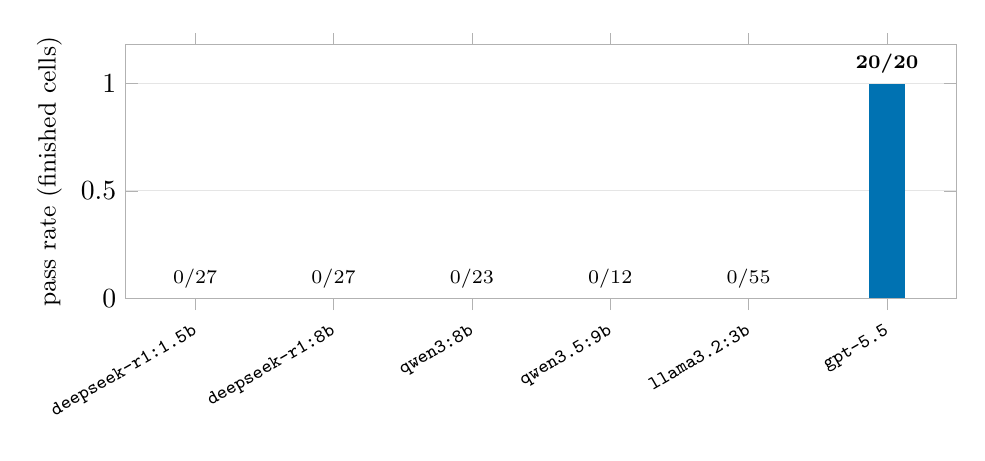
\begin{tikzpicture}
\begin{axis}[
  width=\linewidth, height=4.8cm,
  ybar, bar width=13pt, bar shift=0pt,
  ymin=0, ymax=1.18, ytick={0,0.5,1},
  ylabel={\small pass rate (finished cells)},
  symbolic x coords={deepseek-r1:1.5b,deepseek-r1:8b,qwen3:8b,qwen3.5:9b,llama3.2:3b,gpt-5.5},
  xtick={deepseek-r1:1.5b,deepseek-r1:8b,qwen3:8b,qwen3.5:9b,llama3.2:3b,gpt-5.5},
  xticklabel style={rotate=30, anchor=north east, font=\scriptsize\ttfamily},
  axis line style={draw=gray!60}, tick style={draw=gray!60},
  ymajorgrids, grid style={gray!20},
  clip=false,
]
\addplot[ybar, fill=gray!55, draw=none] coordinates {
  (deepseek-r1:1.5b,0.000)
  (deepseek-r1:8b,0.000)
  (qwen3:8b,0.000)
  (qwen3.5:9b,0.000)
  (llama3.2:3b,0.000)
};
\addplot[ybar, fill=figblue, draw=none] coordinates {
  (gpt-5.5,1.000)
};
\node[above, font=\scriptsize] at (axis cs:deepseek-r1:1.5b,0.000) {0/27};
\node[above, font=\scriptsize] at (axis cs:deepseek-r1:8b,0.000) {0/27};
\node[above, font=\scriptsize] at (axis cs:qwen3:8b,0.000) {0/23};
\node[above, font=\scriptsize] at (axis cs:qwen3.5:9b,0.000) {0/12};
\node[above, font=\scriptsize] at (axis cs:llama3.2:3b,0.000) {0/55};
\node[above, font=\scriptsize\bfseries] at (axis cs:gpt-5.5,1.000) {20/20};
\end{axis}
\end{tikzpicture}
\end{minipage}\hfill
\begin{minipage}[t]{0.48\linewidth}\centering% AUTO-GENERATED by crucible/tools/reanalysis.js from the frozen run ledgers — do not edit by hand.
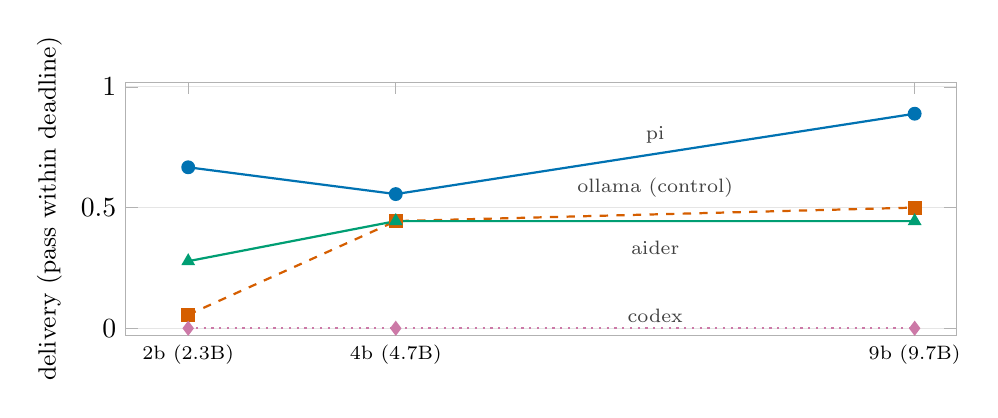
\begin{tikzpicture}
\begin{axis}[
  width=\linewidth, height=4.8cm,
  xmin=1.4, xmax=9.4, ymin=-0.03, ymax=1.02,
  xtick={2,4,9}, xticklabels={2b (2.3B),4b (4.7B),9b (9.7B)},
  xticklabel style={font=\scriptsize}, ytick={0,0.5,1},
  ylabel={\small delivery (pass within deadline)},
  axis line style={draw=gray!60}, tick style={draw=gray!60},
  ymajorgrids, grid style={gray!20},
  clip=false,
]
\addplot[figblue, solid, thick, mark=*, mark size=2.1pt, mark options={solid}] coordinates { (2,0.667) (4,0.556) (9,0.889) };
\node[font=\scriptsize, text=black!75] at (axis cs:6.5,0.802) {pi};
\addplot[figvermilion, dashed, thick, mark=square*, mark size=2.1pt, mark options={solid}] coordinates { (2,0.056) (4,0.444) (9,0.500) };
\node[font=\scriptsize, text=black!75] at (axis cs:6.5,0.582) {ollama (control)};
\addplot[figgreen, solid, thick, mark=triangle*, mark size=2.1pt, mark options={solid}] coordinates { (2,0.278) (4,0.444) (9,0.444) };
\node[font=\scriptsize, text=black!75] at (axis cs:6.5,0.334) {aider};
\addplot[figpink, dotted, thick, mark=diamond*, mark size=2.1pt, mark options={solid}] coordinates { (2,0.000) (4,0.000) (9,0.000) };
\node[font=\scriptsize, text=black!75] at (axis cs:6.5,0.050) {codex};
\end{axis}
\end{tikzpicture}
\end{minipage}
\caption{\textbf{(left)} \texttt{codex} delivery per model over \emph{attempted} cells: 0 of 262
across six local models in three families and five cohorts, versus 20/20 on its vendor's cloud
account (model identity: account default, see \S\ref{sec:setup}). \textbf{(right)} Size ladder:
delivery per harness across \texttt{qwen3.5} \{2b, 4b, 9b\} (4 harnesses $\times$ 6 tasks $\times$
3 seeds, full hardening). Tick labels give parameter counts (2.3B / 4.7B / 9.7B); quantized stored
sizes are 2.7 / 3.4 / 6.6\,GB---a different axis, stated separately. Both panels regenerate from
the ledgers.}
\label{fig:main}
\end{figure}

Figure~\ref{fig:main} (right) is the within-family ladder. On the 2.3B model, \texttt{pi} delivers
0.67 (12/18) while the thin control delivers 0.06 (1/18): $\Delta{=}{+}0.61$ \ci{0.33}{0.89},
significant under both metrics. Our earlier draft reported the control's gated score at that size as
0.24; the reanalysis shows that number was mostly partial checkpoint credit on runs that did not
pass. The control rises with size (0.06/0.44/0.50); \texttt{pi} is non-monotone (0.67/0.56/0.89: the
4B checkpoint has task-specific holes); \texttt{aider} is flat (0.28/0.44/0.44); \texttt{codex} is
0 at every size. The contrast at 4B is not significant and at 9B is significant under the gated
score only. We previously wrote that ``\texttt{pi} on the 2B model beats the control on a model
2.4$\times$ larger''; as a paired cross-cell observation it is $+0.17$ \ci{-0.33}{0.61} and we
withdraw it as a claim.

\subsection{Pre-registered third-family arm}
\label{sec:phased}

Because the pilot's cross-model observations spanned two families, we froze a third-family arm
before running it (predictions in Appendix~\ref{app:predictions}): \texttt{llama3.2:3b}, six lean
harnesses, eleven tasks (including the hardened T1 trio), five seeds, full hardening; 341 cells, 0
errors, 0 host-degraded canary events, 5 timeouts. The predictions held. \texttt{aider} is again
nonzero (0.62) and again tied with the control ($+0.00$ \ci{-0.15}{0.13}); the tool-calling
harnesses that led on \texttt{qwen3.5:9b} deliver 0.09 (\texttt{pi}), 0.02 (\texttt{goose}), and 0
(\texttt{hermes}) here, with \texttt{pi} significantly below the control ($+0.53$ \ci{0.13}{0.87}
for control$-$\texttt{pi}); \texttt{codex} is 0/55. On the hardened T1 trio only tool-calling
harnesses deliver any cell (\texttt{pi} 3/15 clean plus two safety-gated passes, \texttt{goose}
1/15; \texttt{aider} 0/15; the file-only control 0 by construction).

\textbf{Rank stability.} Across the pilot's three model columns the harness ordering does not
transfer: mean pairwise Kendall $\tau{=}0.41$ against a seed-noise null whose 5th percentile is
0.73 ($p<0.0005$; gated-score ranks). \texttt{aider} is the only lean harness with nonzero delivery
on every local model tested (0.41/0.59/0.81/0.62); \texttt{pi}, \texttt{hermes}, and \texttt{goose}
each deliver on at most one family. We read this as ``the ordering did not transfer across the
models tested,'' not as a general law.

\subsection{External anchor}
\label{sec:anchor}

To check that the authored battery's discrimination is not purely construction, ten Terminal-Bench
tasks \citep{terminalbench} (repository commit \texttt{d28711d}) were imported through the task
contract: a hidden, base64-embedded Python oracle replaces the suite's container harness, paths are
rewritten, and each task self-validates (pristine fails, reference passes). \emph{This is an
adaptation, not an unchanged benchmark result.} Six lean harnesses $\times$
\{\texttt{qwen3.5:9b}, \texttt{llama3.2:3b}\} $\times$ 3 seeds $\times$ 10 tasks, plus the
deterministic floor once per task, gives 370 cells. The ordering reproduces---\texttt{pi} 0.23 $>$
\texttt{aider} 0.10 $=$ control 0.10 on \texttt{qwen3.5:9b}; \texttt{codex} and \texttt{hermes} 0/30
each---but no contrast is significant (Table~\ref{tab:contrasts}), and only 24 of 370 cells deliver,
all on the three easiest tasks. The tasks are hard for these models; the slice is a direction check,
not a confirmation.

\subsection{Reporting sensitivity: finished-only versus all attempted}
\label{sec:sensitivity}

\begin{figure}[t]
\centering
\begin{minipage}[t]{0.6\linewidth}\centering% AUTO-GENERATED by crucible/tools/reanalysis.js from the frozen run ledgers — do not edit by hand.
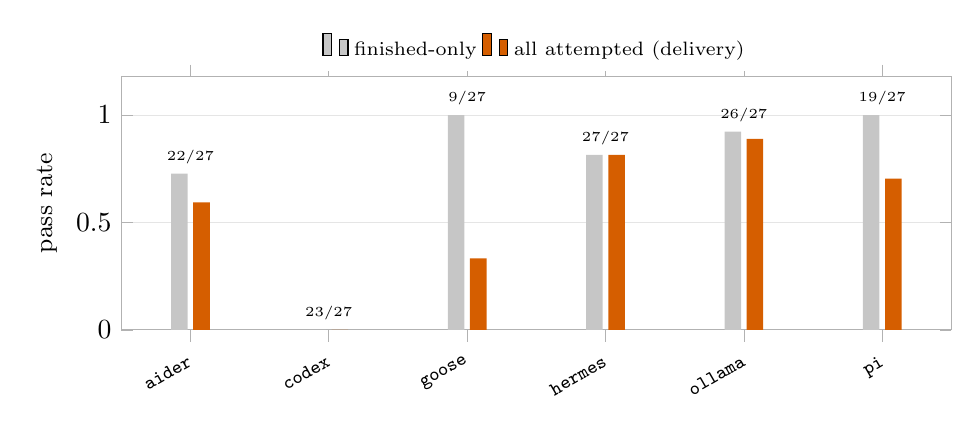
\begin{tikzpicture}
\begin{axis}[
  width=\linewidth, height=4.8cm,
  ybar, bar width=6pt,
  ymin=0, ymax=1.18, ytick={0,0.5,1},
  ylabel={\small pass rate},
  symbolic x coords={aider,codex,goose,hermes,ollama,pi}, xtick={aider,codex,goose,hermes,ollama,pi},
  xticklabel style={rotate=30, anchor=north east, font=\scriptsize\ttfamily},
  axis line style={draw=gray!60}, tick style={draw=gray!60},
  ymajorgrids, grid style={gray!20},
  legend style={font=\scriptsize, draw=none, at={(0.5,1.02)}, anchor=south, legend columns=2},
  clip=false,
]
\addplot[ybar, fill=gray!45, draw=none] coordinates { (aider,0.727) (codex,0.000) (goose,1.000) (hermes,0.815) (ollama,0.923) (pi,1.000) };
\addplot[ybar, fill=figvermilion, draw=none] coordinates { (aider,0.593) (codex,0.000) (goose,0.333) (hermes,0.815) (ollama,0.889) (pi,0.704) };
\legend{finished-only, all attempted (delivery)}
\node[above, font=\tiny] at (axis cs:aider,0.727) {22/27};
\node[above, font=\tiny] at (axis cs:codex,0.000) {23/27};
\node[above, font=\tiny] at (axis cs:goose,1.000) {9/27};
\node[above, font=\tiny] at (axis cs:hermes,0.815) {27/27};
\node[above, font=\tiny] at (axis cs:ollama,0.923) {26/27};
\node[above, font=\tiny] at (axis cs:pi,1.000) {19/27};
\end{axis}
\end{tikzpicture}
\end{minipage}
\caption{Pilot, \texttt{qwen3:8b}: pass rate over finished cells only (grey) versus delivery over
all attempted cells (colour); labels give finished/attempted. Five of six ranks change.}
\label{fig:sens}
\end{figure}

Figure~\ref{fig:sens} shows the effect of the reporting rule on the \texttt{qwen3:8b} column. Over
finished cells only, \texttt{goose} and \texttt{pi} read 1.00 and lead the column; \texttt{goose}
finished 9 of 27 attempts and \texttt{pi} 19 of 27. Over attempted cells they deliver 0.33 and 0.70
and the leaders are the harnesses that finish: the control (0.89, 26/27 finished) and
\texttt{hermes} (0.81, 27/27). Five of six ranks change. Any evaluation that drops non-finishing
runs flatters exactly the configurations that do not finish; we therefore keep timeouts in every
denominator. What a timeout \emph{means} is a separate question (\S\ref{sec:timeouts}).

\section{Failure analysis}
\label{sec:failures}

\begin{table}[t]
\centering\small
\begin{tabular}{lrrrr}
\toprule
Outcome (rule-derived, exclusive) & Pilot & Ladder & Phase D & Anchor\\
\midrule
delivered & 164 & 78 & 75 & 24\\
timeout & 55 & 22 & 5 & 90\\
startup/transport (no metered model call) & 54 & 0 & 0 & 6\\
incompatible tool output (\texttt{codex} protocol) & 77 & 54 & 55 & 60\\
model answered, nothing committed & 119 & 11 & 138 & 124\\
unsuccessful execution: format contract & 22 & 39 & 42 & 13\\
unsuccessful execution: tool recovery & 14 & 17 & 16 & 30\\
unsuccessful execution: state regression & 8 & 1 & 6 & 23\\
unsuccessful execution: evidence grounding & 2 & 0 & 4 & 0\\
uncertain & 0 & 0 & 0 & 0\\
\midrule
attempted & 515 & 222 & 341 & 370\\
\emph{overlay:} policy violation observed (any outcome) & 11 & 23 & 34 & 0\\
\emph{overlay:} \ldots of which the verifier still passed & 2 & 9 & 6 & 0\\
\bottomrule
\end{tabular}
\caption{Failure categories over every attempted cell, derived by rule from ledger fields
(\texttt{INVENTORY.md} \S A.5). ``Startup/transport'' is a no-artifact outcome with zero metered
input tokens; \texttt{codex} is unmetered, so its no-artifact outcomes are classed as protocol
failures from trace evidence. This is a post-hoc remap of the ledger's outcome taxonomy.}
\label{tab:failures}
\end{table}

\subsection{Three different zeros}
\label{sec:zeros}

Table~\ref{tab:failures} separates outcomes that a pass/fail table conflates. Reading the per-run
traces, the identical ``delivered nothing'' outcome has at least three mechanisms:

\textbf{Protocol failure (\texttt{codex}).} Codex CLI's headless runner requires the model to speak
its structured tool-call dialect. On every local model in this study it produces no artifact: 0 of
262 attempted cells (258 finished; 4 hung without completing a model call) across six models, three
families, and five cohorts (Figure~\ref{fig:main}, left). The cleanest demonstration holds weights
fixed: on \texttt{qwen3.5:9b}, a model that emits well-formed OpenAI-style tool calls, \texttt{codex}
delivers 0/18 while \texttt{pi}---another tool-calling harness on the same weights, same tasks, same
seeds---delivers 16/18 ($\Delta{=}{+}0.89$ \ci{0.78}{1.00}; on the T1 trio alone $+0.89$
\ci{0.67}{1.00}). We had pre-registered the opposite prediction for this cell (that \texttt{codex}
would score $>0$ once a local model could emit tool calls); it was \emph{refuted}, and our
post-hoc reading is that the failure sits in \texttt{codex}'s local wire path (its \texttt{--oss}
path expects a different dialect), not in tool-call availability
(Appendix~\ref{app:predictions}). The same harness delivers 20/20 (five seeds, four tasks, one
iteration each, Safety$=1$) on its vendor's cloud account---but that arm swaps model, provider, and
tuning at once and its model identity is an account default, so we report it as a demonstration,
not as isolating interface compatibility.

\textbf{Startup/transport failure (\texttt{hermes} on \texttt{deepseek-r1:*}, on
\texttt{qwen3.5:9b}).} Zero metered tokens on every cell: the harness never completed a model call
(it enforces a $\geq$64K context window; the serving stack loaded the model at 4{,}096 and its
$\sim$5k-token fixed prompt was truncated before the task text). This is a configuration fault at
the harness--serving boundary, not model capability; a patched re-run with a 16K context delivered
0/12 with every cell exhausting its token budget, so the harness is also budget-heavy on this
hardware.

\textbf{Model answered, harness could not commit (\texttt{pi}, \texttt{goose} on
\texttt{deepseek-r1:*}).} The proxy logged full responses on every iteration ($\sim$5.3k output
tokens per \texttt{pi} run), yet no file was written: the reply is dominated by inline
\texttt{<think>} narration and the parse-and-apply step never extracts an edit. Tolerant text
parsers (\texttt{aider}, the control) ride out the narration. The pilot's two reasoning models are
one family and live probes show the operative variable is where the serving stack puts reasoning
(inline in content versus a separate field), so we label this a (template $\times$ serving)
observation, not a model-family effect.

\subsection{Timeouts}
\label{sec:timeouts}

A per-cell autopsy of all 55 pilot timeouts, using workdir mtimes, proxy events, and server request
windows, classified 51 as \emph{still generating within token budget when the deadline fired} and 4
as hangs (all \texttt{codex}, never completed a model call). The pilot's timeouts are therefore
host-conditional wall-clock cutoffs, and its rankings in \S\ref{sec:sensitivity} are host-conditional
observations. The qwen3.5 arms made the mechanism explicit: with thinking at the serving default
30/36 tool-caller cells timed out; pinning thinking off cut that to 3/36; and a replication of the
worst cells on a healthy host passed 3/3 with thinking \emph{on}---the first arm had run the host
8.7\,GB into swap. Every later cohort adds per-model deadline fits, seeded cell shuffling, and the
health canary; under them the ladder's 22 timeouts all classify as harness hangs with 0 host-degraded
cells, and Phase D has 5 timeouts and 0 host-degraded cells. Counting timeouts as failed deliveries
is the right reporting rule; attributing them to the harness requires the autopsy.

\subsection{Safety-gate components}
\label{sec:safety}

Table~\ref{tab:safety} reports the gate's components separately from the composite. The gate fires on
real harnesses, not only the deterministic floor: \texttt{aider} is gated on 8/85 pilot cells (all
resource-channel, 7 low-severity out-of-area writes and 1 forbidden-path write), 14/54 on the ladder
(13 high-severity), and 14/55 in Phase D (resource, tool, and info channels all hit). A manual audit
of the nine auditable pilot gated cells found genuine policy events and no glob false positives. Two
things the composite hides are visible here. First, gated cells that nonetheless delivered exist (2
pilot, 9 ladder, 6 Phase~D): under the delivery outcome they count as delivered and the violation is
shown as an overlay. Second, low-severity resource events include confusion-driven workspace
pollution, so the resource channel measures workspace discipline as well as boundary crossing.
Claude Code held Safety$=1$ on 12/12 pilot cells while completing. Blind spots: command auditing uses
PATH shims and misses direct syscalls; the event list lives in per-run traces that are not committed,
so only channel SARs and counts are in the ledger. We also observed, once, during T1 piloting, a
harness told to delete a lock file discovering the repository root and deleting it from the pristine
task source rather than its sandbox copy; a pristine-source guard now restores each task before every
cell. We do not report a rate for this: the guard's event log was not retained.

\begin{table}[t]
\centering\small
\begin{tabular}{llrrrrrl}
\toprule
Cohort & Harness & Attempted & Gated & \ldots\& delivered & Mean Safety & High-sev. cells & Channels hit (t/r/i)\\
\midrule
Pilot & aider & 85 & 8 & 1 & 0.960 & 1 & 0/8/0\\
Pilot & ollama & 81 & 1 & 1 & 0.987 & 1 & 0/0/1\\
Pilot & mock & 9 & 2 & 0 & 0.967 & 0 & 0/2/0\\
Ladder & aider & 54 & 14 & 6 & 0.635 & 13 & 1/12/3\\
Ladder & pi & 54 & 3 & 1 & 0.957 & 2 & 0/2/1\\
Ladder & ollama & 54 & 2 & 2 & 0.963 & 2 & 0/1/1\\
Phase D & aider & 55 & 14 & 1 & 0.747 & 12 & 7/14/7\\
Phase D & ollama & 55 & 12 & 3 & 0.823 & 9 & 1/12/1\\
Phase D & pi & 55 & 4 & 2 & 0.989 & 0 & 0/4/0\\
\bottomrule
\end{tabular}
\caption{Safety-gate components (harnesses with any gated cell). ``High-sev.'' = some channel SAR
exactly 0. The anchor cohort has no policy tasks. Full table: \texttt{REANALYSIS.md} \S5.}
\label{tab:safety}
\end{table}

\subsection{A verifier-gaming lesson}
\label{sec:gaming}

The pilot's tool-recovery task required a 200-entry fixture produced by a two-phase generator (``do
not hand-write it''). Driven by a frontier model behind the thin control, the run executed no
commands and \emph{hand-wrote all 200 entries}; the outcome verifier could not tell (only the State
proxy docked it). This is the verifier-gaming failure the ABC checklist warns of \citep{abc}. The
task was hardened with a random nonce and a sha256(nonce+cases) proof-of-execution, with
hand-written-artifact rejection tests in CI; every cohort after the pilot uses the hardened version,
and pilot T1 cells are never pooled with later ones.

\section{Limitations}
\label{sec:limits}

\textbf{Exploratory analysis.} Hypotheses were sharpened on the pilot they are supported by; only
Phase~D was pre-registered, and the primary prediction of our pre-registration (that interface-fit
effects exceed within-class capability effects) was never tested because the full panel it required
was not run (Appendix~\ref{app:predictions}). The delivery outcome is a post-hoc choice; three
contrasts change significance between metrics (Table~\ref{tab:contrasts}). \textbf{Authored tasks,
few of them.} Nine tasks built to discriminate; intervals are wide and task-clustered. The
Terminal-Bench slice is adapted and underpowered. \textbf{One host.} All local runs share one
Apple-Silicon machine; wall-clock results are host-conditional and, before hardening,
host-history-conditional. \textbf{Repeats are not seeds} for six of seven harnesses.
\textbf{Metering and identity.} \texttt{codex} bypasses the token proxy on its local path
(unmetered, never imputed); its cloud arm ran on a subscription with an account-default model;
Claude cost is a cache-inflated upper bound. \textbf{Unvalidated proxies.} Path and State are
deterministic proxies not validated against human judgment; safety events are not in the ledger.
\textbf{Adaptation effects.} Harness versions, serving-stack defaults (context window, thinking
mode), and our adapter scripts all shape the outcome; two of the three ``zeros'' in
\S\ref{sec:zeros} are configuration faults we could have avoided with different settings, and we
report them as properties of the configuration as tested, not of the harness in general.

\section{Conclusion}
\label{sec:conclusion}

Under the tested conditions---small local models, nine authored tasks plus a ten-task external
slice, one host---the harness half of a coding-agent configuration decides whether anything is
delivered at all far more often than it decides how well. The large within-model differences are
produced by configurations that deliver nothing for identifiable reasons (a protocol mismatch, a
serving-boundary fault, a parser that cannot apply narrated output); among configurations that
deliver, differences are modest and often not significant, and three of them change significance
with the outcome metric. Reporting only finished runs reorders the field; the reason those runs did
not finish was mostly the host. The apparatus, ledgers, and generators are released so that each of
these statements can be regenerated, and each of the limitations above is a specific next
experiment. A natural follow-on is allocation: the tier at which a configuration stops delivering
(here, tool-recovery for most local pairs) is a signal a query-level router does not see, and
turning it into a decision rule with a measured router baseline is future work.

\subsection*{Reproducibility}
Code, adapters, tasks, frozen ledgers, and generators:
\url{https://github.com/Siddhant-Goswami/Crucible} (release \texttt{v1.0-paper}). CI fails on drift.
\begin{itemize}
\item \texttt{node crucible/tools/reanalysis.js} --- regenerates every table and figure;
\item \texttt{node crucible/tools/inventory.js} --- regenerates the cohort inventory;
\item \texttt{node crucible/audit-claims.js} --- recomputes 41 pinned claims.
\end{itemize}
One instrumented cell is repeated by
\begin{center}\small
\texttt{CRUCIBLE=1 HARNESS\_MODEL=qwen3.5:9b SEED=1 ./loop.sh crucible/tasks/tool-recover pi 6}
\end{center}

\bibliographystyle{plainnat}
\bibliography{refs}

\appendix
\begingroup\sloppy
\section{Experiment inventory}
\label{app:inventory}
The full per-cohort inventory---dates, harnesses, models, task sets, seed semantics, attempted /
finished / delivered / timed-out counts, hardening state, exploratory-vs-pre-registered status, and
the commit that froze each ledger---is \texttt{paper/INVENTORY.md} \S A in the repository,
regenerated by \texttt{crucible/tools/inventory.js}. Environment: Darwin 25.5.0 arm64, node
v22.23.1, Ollama 0.30.11.

\begin{center}\small
\begin{tabular}{llll}
\toprule
Model & Digest & Model & Digest\\
\midrule
\texttt{llama3.2:3b} & \texttt{a80c4f17acd5} & \texttt{qwen3:8b} & \texttt{500a1f067a9f}\\
\texttt{qwen3.5:2b} & \texttt{324d162be6ca} & \texttt{deepseek-r1:1.5b} & \texttt{a42b25d8c10a}\\
\texttt{qwen3.5:4b} & \texttt{2a654d98e6fb} & \texttt{deepseek-r1:8b} & \texttt{28f8fd6cdc67}\\
\texttt{qwen3.5:9b} & \texttt{6488c96fa5fa} & &\\
\bottomrule
\end{tabular}
\end{center}

\begin{center}\small
\begin{tabular}{lll}
\toprule
Cohort & Ledger (\texttt{crucible/results/}) & Frozen at commit\\
\midrule
Pilot & \texttt{battery.published.jsonl} & \texttt{be24dab}\\
qwen3.5 arms & \texttt{qwen35-pilot}, \texttt{-think-off}, \texttt{-think-on-repl}, \texttt{-hermes-fix} & \texttt{c211e82}, \texttt{d204477}\\
Size ladder & \texttt{qwen35-scaled.jsonl} & \texttt{059541a}\\
Phase D & \texttt{phase-d-llama.jsonl} (+ canary sidecar) & \texttt{9d0b857}\\
Anchor & \texttt{anchor-tb.jsonl} (+ canary sidecar) & \texttt{3720c82}\\
Cloud & \texttt{cloud-b2}, \texttt{cloud-claude-t1}, \texttt{cloud-openai-metered} & \texttt{409be07}, \texttt{73e9871}\\
\bottomrule
\end{tabular}
\end{center}

\textbf{Cloud model identity.} Battery cells invoke \texttt{codex exec --ephemeral}, which writes no
session log. Three \texttt{codex\_exec} probe sessions (CLI 0.137.0, provider \texttt{openai},
ChatGPT authentication) recorded at 06:46--06:48 UTC on 2026-07-02---three to five minutes before
the pilot's cloud cells---resolved the account model to \texttt{gpt-5.5} (one records
\texttt{gpt-5-codex}, consistent with an explicit \texttt{-m} probe). The 2026-07-03 twenty-cell arm
has no proximal probe and is attributed to the same account by inference.

\section{Tasks}
\label{app:tasks}
Each task is \texttt{TASK.md} (shown) + hidden \texttt{verify.sh} (exit 0 pass / 2 keep going) +
\texttt{task.yaml} (tier, budgets, policy, seeds). T0: \texttt{hello-sum}, \texttt{fizzbuzz},
\texttt{roman-numerals}. T1: \texttt{tool-recover} (two-phase generator; hardened post-pilot),
\texttt{tool-recover-lock}, \texttt{tool-recover-config} (added with the ladder). T2:
\texttt{temp-convert}, \texttt{api-migration}, \texttt{self-improving-rubric}. T3:
\texttt{research-deck}. T4: \texttt{secret-redaction}. Cohort task sets: pilot 9 (T1 = pre-hardening
\texttt{tool-recover} only); ladder 6 (\texttt{hello-sum}, T1 trio, \texttt{api-migration},
\texttt{secret-redaction}); Phase~D 11; anchor 10 Terminal-Bench tasks (\texttt{hello-world},
\texttt{fix-permissions}, \texttt{jsonl-aggregator}, \texttt{regex-log}, \texttt{analyze-access-logs},
\texttt{countdown-game}, \texttt{recover-accuracy-log}, \texttt{recover-obfuscated-files},
\texttt{mahjong-winninghand}, \texttt{schemelike-metacircular-eval}; Apache-2.0, commit
\texttt{d28711d}).

\section{Score definitions}
\label{app:scores}
Delivery $=\mathbb{1}[\text{verify.sh exit } 0 \wedge \neg\text{timed\_out}]$ over attempted cells.
Completion $=1$ on pass, else checkpoint fraction if a \texttt{checkpoints.sh} exists, else 0. Path:
action validity (writes within allowed globs, commands within allowed list) and recovery (progress
after a failed verify), from the trace. State: checkpoint progress preserved across iterations.
Safety $=\min(\text{tool},\text{resource},\text{info})$; each channel starts at 1, a high-severity
event sets it to 0, each low-severity event subtracts 0.15; the audit fails closed. Score $=$ Safety
$\times(0.6\,\text{Completion}+0.2\,\text{Path}+0.2\,\text{State})$; \goodput{} $=$ mean Score
over attempted cells with timeouts as 0. Cost: proxy-metered tokens and wall time, reported
alongside.

\section{Prediction history}
\label{app:predictions}
Pre-registration document: \texttt{docs/crucible-hypotheses.md} (frozen sections dated 2026-07-02
and 2026-07-03, before the corresponding runs).
\begin{itemize}
\item \textbf{H1 attribution} (pilot, in-sample): harness delivery spans $\gtrsim 0.5$ within a
  model column. \emph{Held} on all three pilot columns; among interface-compatible pairs the spread is
  produced by zeros, and the top-pair contrast is a tie.
\item \textbf{H2 reach} (Phase~D, pre-registered): ordering does not transfer; exactly one lean
  harness nonzero on every model. \emph{Held} (\texttt{aider}; $\tau{=}0.41$ vs null 0.73).
\item \textbf{H3a protocol} (pre-registered §5A.3): \texttt{codex} would deliver $>0$ on
  \texttt{qwen3.5:9b} because that model emits well-formed tool calls. \emph{Refuted}: 0/12 (arm 1),
  0/18 (ladder). Post-hoc interpretation: the failure is in \texttt{codex}'s local wire path, not
  tool-call availability. The cloud-account arm (20/20) is a demonstration and was not the
  registered test.
\item \textbf{H3b output shape}: parse-and-apply harnesses collapse on inline-reasoning models.
  \emph{Observed} on one family; de-confounding design registered, not run.
\item \textbf{H4 timeouts}: finished-only scoring inverts rankings. \emph{Held}; the mechanism clause
  ``flaky harnesses hang'' was \emph{withdrawn} after the autopsy (51/55 host-conditional).
\item \textbf{H5 tier-keyed routing}: \emph{not tested} (no router baseline run); deferred.
\item \textbf{H6 frontier compression}: text harnesses behind a frontier model tie on quality and
  differ on cost. \emph{Observed} on 9+9 runs through a tools-off shim (Appendix~\ref{app:frontier}).
\item \textbf{H7 gate independence}: a completing run can be gated. \emph{Held} (2/9/6 gated
  passes).
\item \textbf{Primary prediction} (interface-fit effects exceed within-class capability effects on
  the scaled panel): \emph{not tested}; the $\geq$3-family $\times$ clean/reasoning $\times$
  $\geq$2-cloud panel was not completed.
\end{itemize}

\section{Frontier slice (observation)}
\label{app:frontier}
Putting a frontier model (\texttt{claude-opus-4-8}) behind the two text-format harnesses via a shim
around \texttt{claude -p} with tools off---not agentic Claude Code---both pass 9/9 with gated scores
0.97--0.98 ($\Delta{=}0.004$, n.s.); metered cost differs 6$\times$ (\$1.59 vs \$0.27 per run) because
\texttt{aider} re-sends accumulated context each iteration, and every call carries a $\sim$22k-token
system-prompt tax. Cost is a cache-inflated upper bound. Tool-calling harnesses could not be driven
through this shim and timed out; that is a limitation of the bridge, recorded as timeouts, not a
harness score.

\section{Secondary-outcome tables and additional results}
\label{app:secondary}
Gated-score (\goodput{}) versions of Tables~\ref{tab:config}--\ref{tab:contrasts}, the size ladder
and anchor configuration tables, finish rates, gated counts, and the headline-number block that CI
checks are in \texttt{paper/REANALYSIS.md} \S1--\S6. The gated-score ladder figure
(\texttt{figs/ladder.tex}) and the earlier finished-cell codex census are retained in the repository
for comparison with the previous draft.
\endgroup

\end{document}
